\subsection{CERN and LHC} \label{subsec:LHC}
After Second World War, Europe was tore apart and its science was no longer world-class. As a reaction to this, French physicist Louis de Broglie put forward the first official proposal for the creation of a European laboratory at the European Cultural Conference, which opened in Lausanne on 9 December 1949. In 1952, with the mandate of establishing a world-class fundamental physics research organization in the continent, a provisional body was founded in 1952. On the 29$^{th}$ September 1954, the \textit{Conseil Européen pour la Recherche Nucléaire} (European Council for Nuclear Research, CERN) was founded by 12 countries. Despite the early change of the name to \textit{European Organization for Nuclear Research}, the acronym remains unchanged until nowadays. Based in Geneva, currently it is the world largest particle physics center and it includes 22 member states.

Several scientific achievements have been made through CERN experiments, for instance: the discovery of neutral currents~\cite{hasert1974observation}, the W and Z bosons~\cite{Watkins:1986va}, the determination of the number of light neutrino families~\cite{decamp1989determination}, the direct discovery of CP violation~\cite{Fanti:1999nm} or Higgs boson discovery~\cite{Carmi:2012in}.

Aproved by CERN Council in 1994 and started for first time in 2008, the Large Hadron collider (LHC) is the world's newest and most powerful tool for Particle Physics research~\cite{Evans:2008zzb}. The LHC is a two-ring super accelerator proton-proton collider built along the $27$~km of LEP, the electron-positron accelerator used in CERN from 1989 to 2000~\cite{Myers:1991ym}. The aim of the hadronic collider was to discover the Higgs boson, which was achieved in 2012, as well as to study rare events. 
It is designed to collide two beams of hadrons, mainly protons,
with a centre-of-mass energy of the collision of $\sqrt{s}=14$~TeV and an instantanius luminosity of $10^{34}$~cm$^{-2}$s$^{-1}$. Apart from protons, it can also collide heavy (Pb) ions with an energy of 2.8 TeV per nucleon and a peak luminosity of $10^{27}$~cm$^{-2}$s$^{-1}$ \cite{muller2012first}. An scheme of LHC and its injection system can be seen in Figure~\ref{Fig:LHC}.

\begin{figure}[htb]
\centering
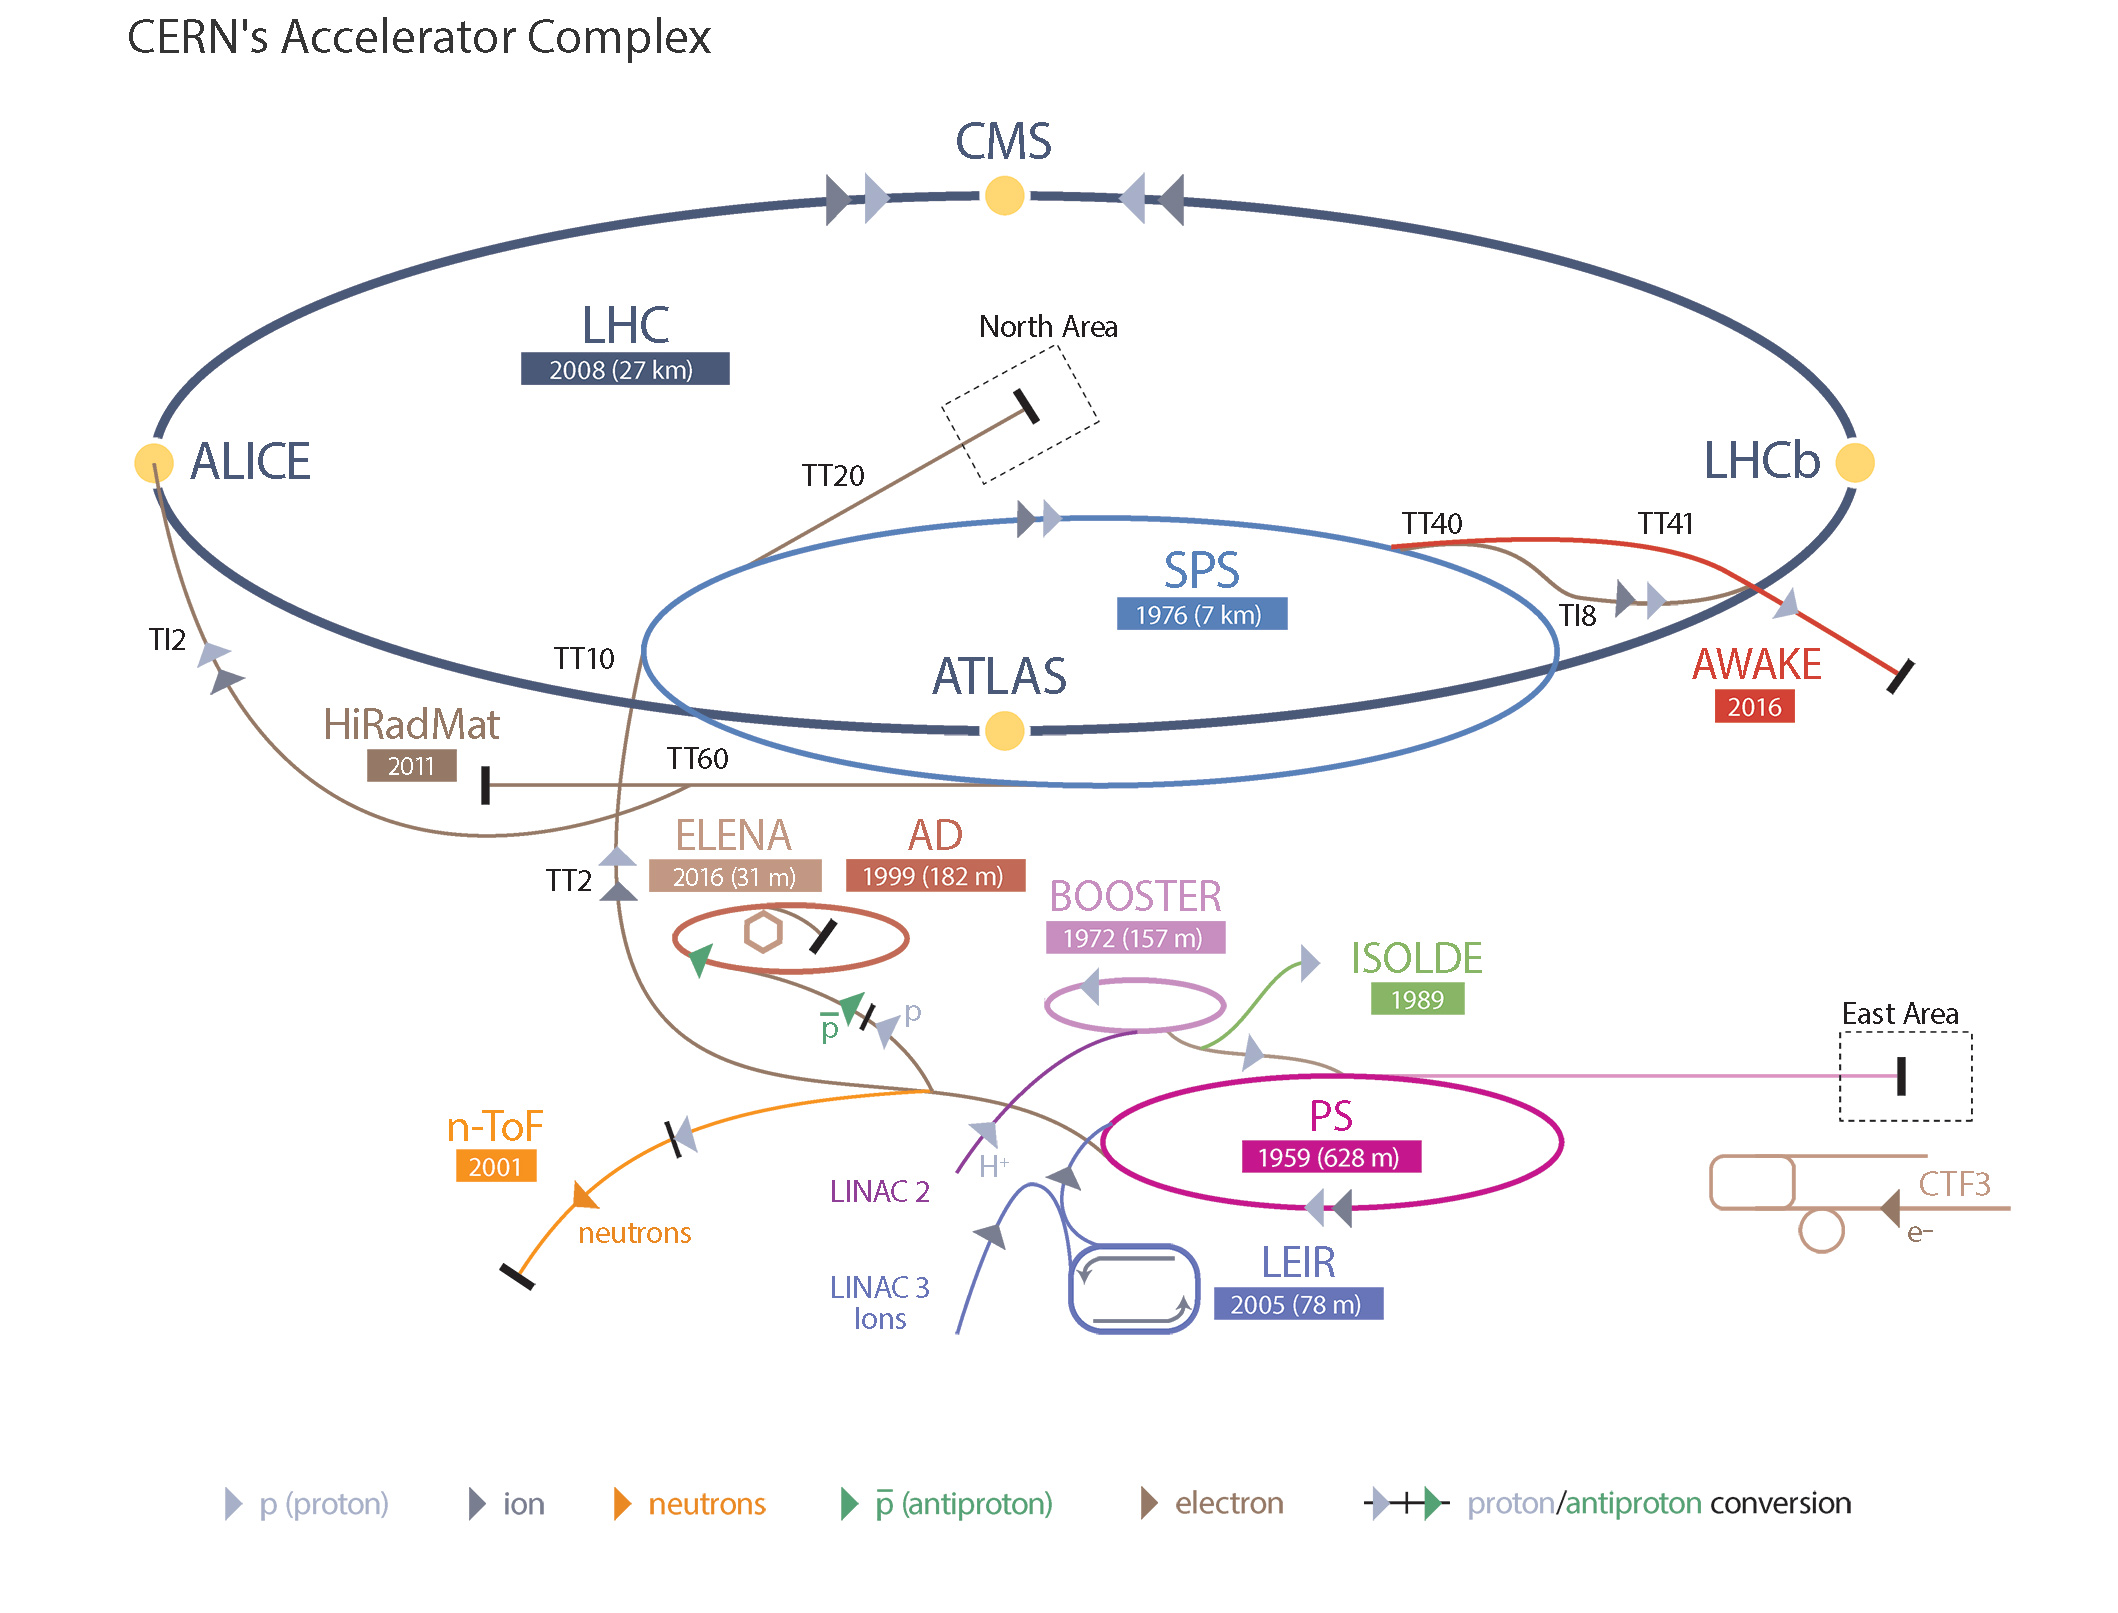
\includegraphics[width=0.85\textwidth]{/afs/ific.uv.es/user/p/pamarag/public/RedaccionTFM/Figuras/LHC_default.jpg}
\caption{Scheme of CERN accelerator complex.}
\label{Fig:LHC}
\end{figure}

The proton bunches are produced ionizing hydrogen atoms and then sent through a series of preaccelerators that boost the hadrons until they have an energy\footnote{Minimum energy at which the LHC can maintain a stable beam.} of 450~GeV. At this point, two sets of proton beams are injected in the LHC pipes in opposite directions. The beams keep aligned and stable thanks to the superconducting dipoles and quadrupole magnets% with a field of up to $8.3$~T
. Once the protons are in the main rings, their energy is raised by increasing the intensity of the magnetic field from 0.54~T to 8.3~T. If the energy is maintained, the beams are declared stable and the different experiments start the data taking. The beams collide at the points where the detectors are located during periods of time of 24~h or less. The beams stop circulating through the rings when they lose stability or the losses of protons due to the collisions make the quality of the beams insufficient. At this stage the beam is directed out of the accelerator and the magnets ramped down to 0.54~T.

There are four main experiments in the LHC (ATLAS, CMS, LHCb and ALICE) and two smaller (TOTEM and LHCf). All of them sit underground in huge caverns on the LHC ring. The biggest of these are ATLAS and CMS~\cite{Chatrchyan:2008aa}, which use general-purpose detectors to investigate the largest range of physics possible. CMS and ATLAS detectors are independently designed to ensure a real cross-checking of new discoveries. ALICE, LHCb, TOTEM and LHCf have detectors specialized on specific phenomena. ALICE~\cite{aamodt2008alice} is dedicated to heavy ion (Pb-Pb) experiments, LHCb~\cite{alves2008lhcb} searches for $b$-physics, TOTEM~\cite{anelli2008totem} does for protons from elastic scattering at small angles and LHCf~\cite{adriani2008lhcf} does for neutral pions produced in the forward direction. There is a minor experiment hold at LHC that worth to be mentioned, MoEDAL, which uses detectors deployed near LHCb to search for the magnetic monopole~\cite{pinfold2009technical}. The simulated events used for this project are generated for the ATLAS detector, explained in section~\ref{subsec:ATLAS}.

\subsubsection*{Performance}
An important feature of LHC operation is the luminosity, which measures the number of collisions produced by the accelerator. The instantaneous luminosity ($\mathcal{L}_{ins}$) provides the rate of events given the cross section ($\sigma_{event}$) of the event under study:
\begin{equation*}
\frac{dN_{event}}{dt}=\mathcal{L}_{ins} \cdot \sigma_{event}
\end{equation*}
If two bunches containing $n_1$ and $n_2$ particles collide head-on with the frequency of bunch crossing $f$ , a basic expression for the luminosity is~\cite{Hoecker:2016vvy}:
\begin{equation*}
\mathcal{L}_{ins} = f \cdot \frac{n_1 n_2 n_b}{4\pi \sigma_x \sigma_y}\cdot F(\theta_c ,\sigma_x, \sigma_z)
\end{equation*}
At the LHC, $f$ has a value of $f=11 245.5$~Hz, calculated from its length (27 km) and assuming that the particles there travel at the speed of light. The maximum number of proton bunches in the machine with 25~ns slots is $n_b=2808$; the theoretical maximum of 3564 bunches cannot be reached due to space needed between bunch trains and for the beam dump kicker magnets. The $n_1 \approx n_2 \approx  1.15 \times 10 ^{11}$. $\sigma_x \approx \sigma_y  \approx 12,...,50$ $\mu$m are the rms transverse beam sizes in the horizontal and vertical directions, this characterize the beam optics. Finally, the factor $ F(\theta_c ,\sigma_x, \sigma_z)$ accounts for luminosity reduction due to the beam crossing angle $\theta_c$. As can be seen, $\mathcal{L}_{ins}$ only depends on the machine and its beam parameters~\cite{Olive:2016xmw}.

During the first proton run, that took place between 2010 and 2013, the experiment was carried out at 3.5~TeV with a bunch spacing of 50~ns instead of the 25 ns. This implied fewer bunches with larger intensity and hence a high peak luminosity but larger pileup than nominal. Run~I resulted in about 30~fb$^{-1}$ of proton data (which was used for the Higgs boson discovery). Run~I was followed by a long shutdown (LS1, 2013–2014) with a large number of consolidation and upgrade activities. Run 2 started in 2015 and is planned to continue until the end of 2018. The main accelerator goals of
Run 2 are to produce more than 100~fb$^{-1}$ of data. The parameter archived (by June 2016) are shown in Table~\ref{table:LHCParameters}~\cite{bruce2016lhc}. Figure~\ref{Fig:Lumi} shows the integrated delivered luminosity per year in the LHC.


\begin{table}
\begin{tabular}{|l | c c c c c c|}
\hline
                 & Design & 2010 & 2011 & 2012 & 2015 & June 2016 \\ \hline
Beam energy (TeV) & 7.0 & 3.5 & 3.5 & 4.0 & 6.5 & 6.5 \\ \hline
Protons/Bunch ($\times 10^{11}$) & 1.15 & 1.0 & 1.3& 1.5&1.1&1.1 \\ \hline
Maximum number of bunches & 2808 & 368  & 1380  & 1380 & 2244 & 2076\\ \hline
Bunch spacing (ns) & 25 & 150 & 50 & 50 & 25 & 25 \\ \hline
Maximum peak luminosity ($\times 10^{11}$ cm$^{-2}$s$^{-1}$) & 1.0 &0.021&0.35&0.77&0.51&1.01\\ \hline
Total integrated luminosity (fb$^{-1}$) & &0.048&5.5&22.8&4.2&8.1\\ \hline
\end{tabular} 
\caption{Parameters of LHC during Run~I and Run~II (unitil June 2016)~\cite{bruce2016lhc}.}
\label{table:LHCParameters}
\end{table}


  
\begin{figure}[htb]
\centering
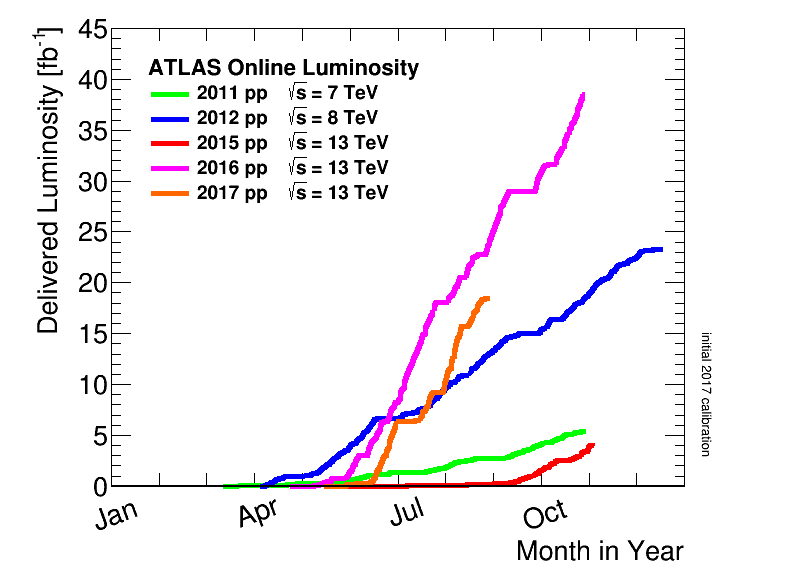
\includegraphics[width=0.70\textwidth]{/afs/ific.uv.es/user/p/pamarag/public/RedaccionTFM/Figuras/intlumivsyear.png}
\caption{Cumulative luminosity versus day delivered to ATLAS during stable beams and for high energy p-p collisions~\cite{Web:Luminosity}.}
\label{Fig:Lumi}
\end{figure}
%https://twiki.cern.ch/twiki/bin/view/AtlasPublic/LuminosityPublicResultsRun2




\subsection{The ATLAS detector} \label{subsec:ATLAS}
 % https://atlas.cern/discover/detector
The ATLAS (A Toroidal LHC ApparatuS) detector, which gives the name to the experiment and collaboration, is the largest volume detector ever constructed for a particle collider. It investigates a wide range of physics, from the search of extra dimensions to dark matter. Sat in a cavern 100~m below ground, it has the dimensions of a cylinder, 46 m long, 25 m in diameter. The ATLAS detector weighs $7.000$ tonnes\footnote{This is similar to the weight of the Eiffel Tower.}.

As can be seen in Figure~\ref{Fig:ATLAS}, ATLAS detector is composed by six different subsystems: The Inner Detector sorrounded by the Solenoidal Magnet, the Electromagnetic and Hadronic calorimeters, the Toroid Magnets and the Muon Spectrometer~\cite{ATLAS:1999uwa}.

\begin{figure}[htb]
\centering
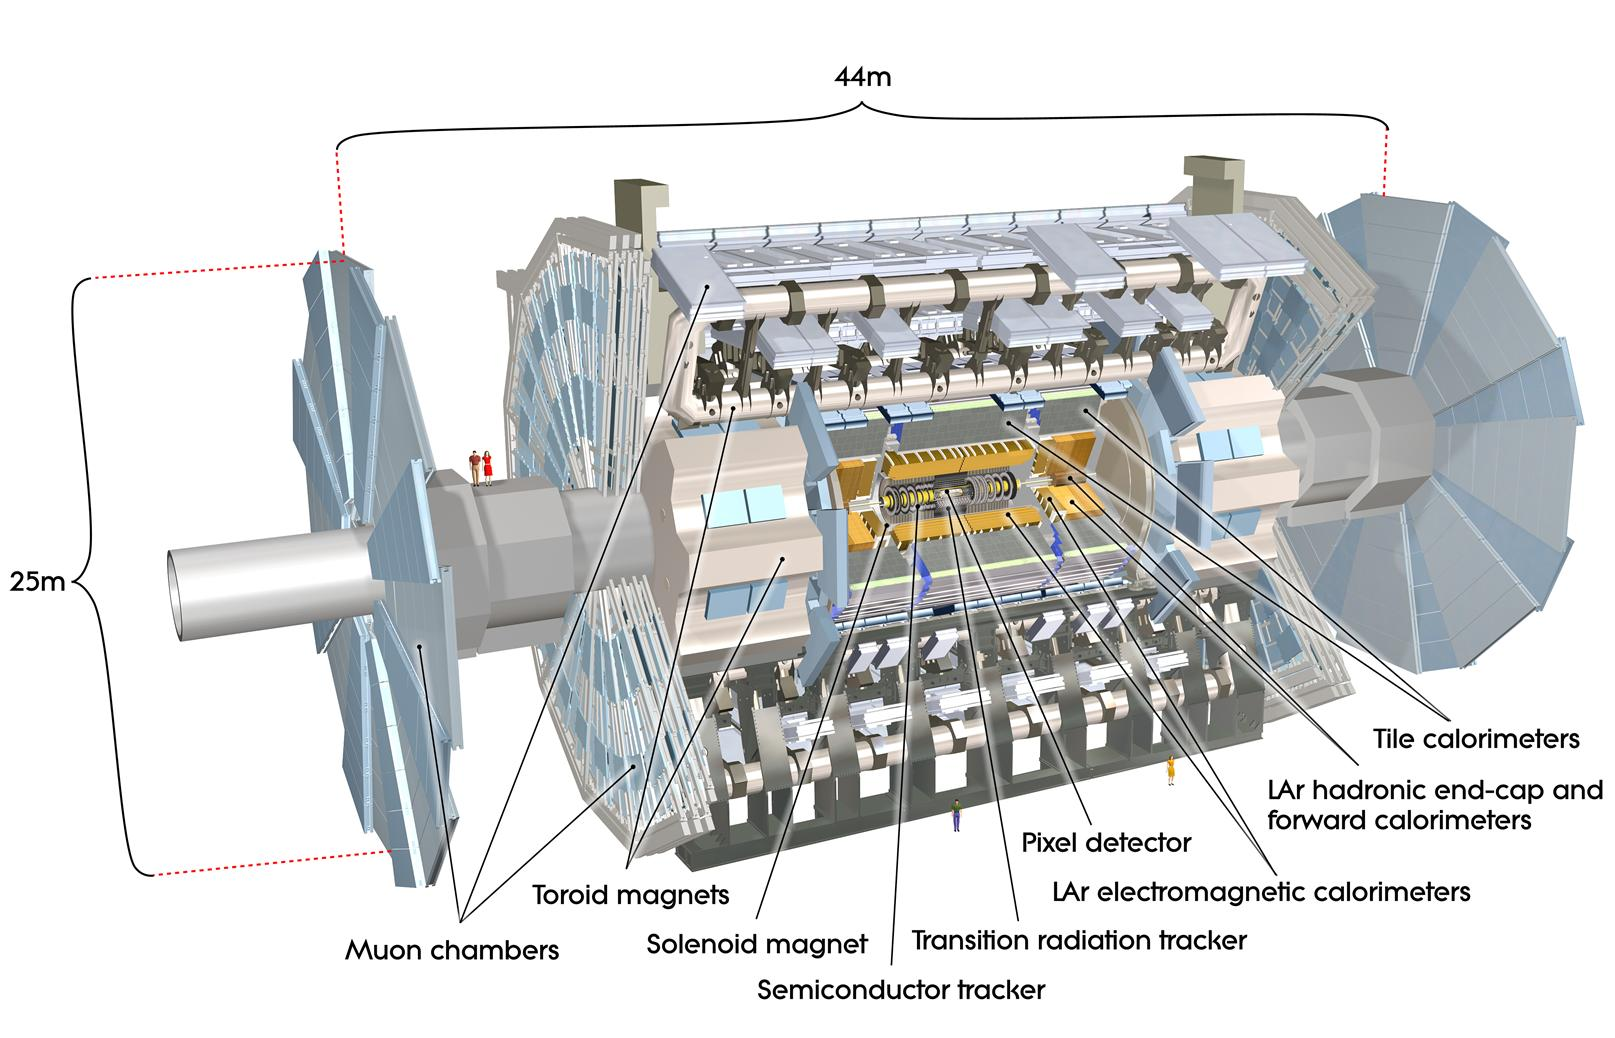
\includegraphics[width=0.9\textwidth]{/afs/ific.uv.es/user/p/pamarag/public/RedaccionTFM/Figuras/figures_AtlasDetectorLabelled.png}
\caption{The ATLAS detector layout with all its subdetectors.}
\label{Fig:ATLAS}
\end{figure}

The coordinate system of ATLAS has its origin at the collision point, at the center of the detector. The beam axis defines the $Z$-axis, the direction from the origin to the center of the ring gives the $X$-axis and the orthogonal to the others axis is the $Y$-axis, which points upwards. The azimuthal angle, $\phi$, is measured around the $X$-axis and the polar angle, $\theta$, respect to the beam axis. The latter is used to define the pseudorapidity (Figure \ref{Fig:Pseudorapidity}), which is a purely geometrical quantity that depends on the polar angle $\theta$, but not on the particle’s mass:
\begin{equation}
\eta = -ln \tan\left(\frac{\theta}{2}\right)
\end{equation}

\begin{figure}[htb]
\centering
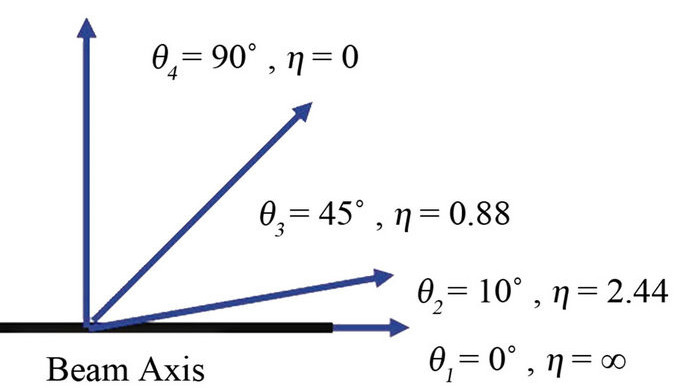
\includegraphics[width=0.5\textwidth]{/afs/ific.uv.es/user/p/pamarag/public/RedaccionTFM/Figuras/pseudora.jpg}
\caption{Pseudorapidity ($\eta$) values on a polar plot. A $\theta=0$ corresponds to the beam axis.}
\label{Fig:Pseudorapidity}
\end{figure}

The forward part of the detector is the one with large values of $|\eta|$. The part of the detector with $Z>0$ is called \textit{Side A}, while $Z<0$ is named \textit{Side C}. The subsystems parallel to the $Z$-axis form what is called the barrel of the detector. On the two sides of the barrel there are the end-caps, these are the detecting elements which are arranged in transversal planes to the beam axis.

\subsubsection*{Inner detector}
The inner detector (ID) is the innermost part of the detector. Beginning only a few centimetres from the proton beam axis, consists in a cylinder with a radius of $1.05$~m and a length of 7~m. It is intended mainly to detect charged particles inside the range $|\eta|<2.5$, revealing its position and momentum, i.e. to reconstructs its traces. It is also used to identify the type of particle, reconstruct the primary vertices and particles such as electrons or jets from $b$-quark hadronization. 
It is composed of three different and independent subdetectors: the Pixel detector and the semiconductor tracker (SCT), which are precision tracking detectors, and the straw tubes of the transition radiation tracker (TRT). The general function of each system is to record a ``hit" when a particle passes through a certain point across it. The momentum resolution of the ID is $\frac{\sigma_{pT}}{p_T}=0.05 \% \oplus 1 \%$ for $p_T <1$~TeV.

\begin{itemize}
\item Pixel detector: It is innermost part of ID. Having a high granularity, it provides a very high precision set of measurements close to the interaction point. Contains four layers in the barrel and three disks on each end-cap; in total there are $1744$ modules with size of 2~cm by 6~cm. The material for the detection is semiconductor silicon.
\item SCT: The next part is conceptually similar but with long and narrow strips of 80~$\mu$m by $12.6$~cm instead of pixels, which translates into a larger coverage area. Since it measures particles over a much larger volume than the previous layer, it is the most important part of the detector when it comes to track the particles in the plane perpendicular to the beam.
\item TRT: The last part of the ID is formed by layers of gaseous straw tube elements and transition radiation material. The TRT provides electron identification capability through the detection of transition radiation X-ray photons.
%The drift tubes have 4 mm of ciameter and the estraw 
\end{itemize}

\subsubsection*{Calorimeter}
The energy of the particles is measured by the calorimeters. Situated outside the solenoidal magnet that surrounds the ID, the calorimeter covers all the azimuthal angle and a range of $|\eta|<4.9$. Its basic function is to absorb the energy of both charged and neutral particles in order to measure it. This part of ATLAS is divided in two subdetectors: an inner electromagnetic calorimeter (ECal) and the hadronic one (HCal).

The calorimeters use alternating layers of absorber and active material. The incident particle produces a shower of secondary particles when it interacts with the material. The energy of the showers is detected when it is deposited in the active material. Liquid Argon (LAr) was chosen as the main active material for the calorimeter due to its intrinsic linear behaviour and radiation hardness, other parts use plastic scintillators. The only particles that scape from calorimeters are the muons and the neutrinos; the former ones are detected in the muon system and the latter leaves the detector without interacting.
%but the presence of neutrinos can be inferred through the missing transverse energy
\begin{itemize}
\item[ECal]: It is the inner of the two calorimeters. Its barrel region provides high granularity for precision measurements of electrons, positrons and photons. Mostly made by LAr, the ECal absorbs energy from particles that interact electromagnetically (photons and electrically charged). The showers in the LAr liberate electrons that are collected and recorded later. The barrel part covers $|\eta|<1.475$ and the two endcap components cover a range of $1.375<|\eta|<3.2$. It has great precision in the location of the energy deposition and its amount. The expected energy resolution of the ECal is $\frac{\sigma_E}{E}=\frac{10 \%}{\sqrt{E}} \oplus 0.7 \%$ in the energy range $10 < E< 245$~GeV.

\item[HCal]: Surrounding the ECal there is the HCal, which provides information about the particles that pass through the latter and are strongly interacting (the hadrons). This calorimeter is less precise in magnitude and location than the ECal. It is composed by three subdetectors: a Tile calorimeter (TileCal), a LAr hadronic endcap (HEC) and LAr forward calorimeter (FCal).
\begin{itemize}
\item[TileCal]: Placed directly outside the ECal, it covers $|\eta|< 1.7$. Its active material is scintillating plastic tiles and its absorber is steel. The tiles are illuminated by the hadronic showers and the light is recorded. The expected energy resolution for the barrel and endcap calorimeters is $\frac{\sigma_E}{E}=\frac{50 \%}{\sqrt{E}} \oplus 3 \%$ for single pions of energy $10 < E< 300$~GeV.
\item[HEC]: It consists of four wheels, two in each endcap, built from parallel copper plates with 8.5 mm LAr gaps. It overlaps with the forward calorimeter in the range of $3.1 <|\eta|<3.2$ and with the TileCal in $1.5 <|\eta|<1.7$.
\item[FCal]: Situated near the pipe ($3.1<|\eta|<4.9$), consists of three modules in each endcap: A copper one for electromagnetic measurements and two of tungsten for hadronic energy interactions measurements. Its expected energy resolution is $\frac{\sigma_E}{E}=\frac{100 \%}{\sqrt{E}} \oplus 10 \%$ for single pions in $10 < E< 300$ GeV energy range.
\end{itemize}
\end{itemize}
 
\subsubsection*{Muon system}
The Muon Spectrometer (MS) is the outermost part of the ATLAS detector and its aim is to detect charged particles escaping from the barrel and endcaps calorimeters. The MS measures the momentum of these particles in the $|\eta|<2.7$ range. Muons are the only particles that can reach the MS and be detected. The MS measures the trajectories of the muons to determine its momentum and charge sign with precision. This measurement takes place inside a magnetic field produced by superconducting toroid magnets. The muon chambers are made of thousands of metal tubes equipped with a central wire and filled with gas. When a muon passes through the these tubes, it leaves a trail of electrically charged ions and electrons which drift to the sides and center of the tube. The position of the muon is, therefore, determined from the time that it takes to these charges to drift.
The MS is equipped with four different kind of chambers: Monitored Drift Tube chambers, Cathode Strip Chambers, Resistive Plate Chambers and Thin Gap Chambers. The first two are used for precision measurements of mass and the other for the trigger and data acquisition. It is designed to achieve a resolution below $4 \%$ for muons with transverse momentum $p_T < 2$~GeV, if $p_T = 1$~TeV the resolution increases to $10 \%$.

%hey collide at the center of the detector 40 million times per second (i.e. 40 MHz or every 25 ns). 
\subsubsection*{Trigger and data acquisition system} \label{subsec:trigg}
The proton bunches travel almost at the speed of light and they collide at the center of the detector 40 million times per second, i.e. 40 MHz or every 25 ns. Since reading out and storing all the information ($\sim 100$ TB/s) is not feasible, ATLAS uses a complex and highly distributed Trigger and Data Acquisition (TDAQ) system, in charge of selecting only interesting data and transporting those to permanent mass storage ($\sim 1$ GB/s) for later analysis. This reduction is carried out in two stages: The electronic performs a initial selection and then a large computer farm analyses the data that pass the initial filter.

ATLAS subdetectors make several filterings. The Level~1 (L1) Trigger performs a first rejection based on simple calorimetry and muon tracking information by reducing the data by a factor of 100. It is a hardware trigger that decreases the amount of information accepted rate to 75~kHz. After the L1 the data is stored in large memory buffers ($\sim 17 \times 10^{3}$ cores) in the Read-Out system (ROS) for further real time analysis in the High Level Trigger (HLT) farm. The HLT is consists in two steps. The first step is the L2, that uses the regions of interest defined by L1 to further reduce the event rate to 1~kHz. The second step is the event filter, which has access to full detector granularity and reduces the output to approximately 400~Hz. The surviving data is stored for later physics analyses~\cite{Astigarraga:2015caa}.
